

\chapter{Resolução de sistema com posto incompleto}
Para o teste do posto incompleto, foi gerado $Ax = b$ onde:


\[
A =
\left(
\begin{array}{ccc}
	1.0000000 & 0.0000000 & 1.0000000\\
	2.0000000 & 5.0000000 & 2.0000000\\
	-1.0000000 & -5.0000000 & -1.0000000\\
	-1.0000000 & 0.0000000 & -1.0000000\\
\end{array}
\right)
\]
\[
b =
\left(
\begin{array}{c}
10.000  \\
45.000  \\
-35.000  \\
-10.000  \\
\end{array}\right)    
\]
com valores pré-determinados\[ x = 
\left(
\begin{array}{c}
6\\
5\\
4\\
\end{array}
\right)\]

Note que a terceira e a quarta linha sao combinações lineares da primeira e segunda linha.
Enviando a matriz A e o vetor b para o programa (arquivo postoinc.txt), obtemos o resultado $x_0 = 10$ ~e~ $x_1 = 5$, com resíduo 16.44817.

A solução é razoável, uma vez que a matriz A é singular, porém não é a melhor solução gerada, pois a encontrada pelo programa apresenta o resíduo de 16.448, enquanto o resíduo com o sistema utilizando $x_1$ é zero.




\chapter{Resolução de sistema com posto completo e problema dos quadrados mínimos}
Inicialmente foi tomado o polinômio $x^5-7x^4+5x^3-3x^2+2x-1$ e sorteados
70 pontos para servirem como  dados de entrada e foram calculadas as funções que
melhor aproximariam esses pontos.
As funções soluções foram encontradas em diferentes graus. 

Após, os dados foram perturbados em 15\% e foram calculadas novas
soluções. Estas funçoes e suas características de aproximação estão descritas 
a seguir.

\section{Dados iniciais}
Os pontos sorteados e a função caracterizadas pelo polinômio \[x^5~-~7x^4~+~5x^3~-~3x^2~+~2x~-~1\]
estão plotados abaixo.

\begin{figure}[h]
\centering
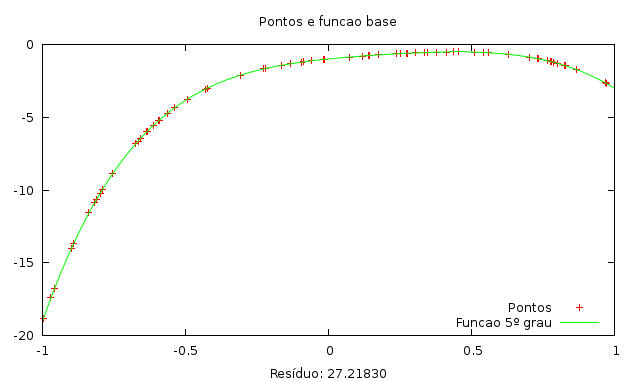
\includegraphics[scale=0.7]{funcbase}
\end{figure}

Os pontos foram usados para buscar funções que os atravessassem reduzindo o resíduo.
A partir dessas soluções, os dados foram perturbados e suas novas funções calculadas.



\newpage
\section{Solução 2º grau}

Ao buscar uma função de grau 2 para aproximar os pontos encontrou-se os seguintes 
coeficientes:

\(x_0 = -3.74052 ~$e$~  x_1 = 5.87079 \)

\begin{figure}[h]
\centering
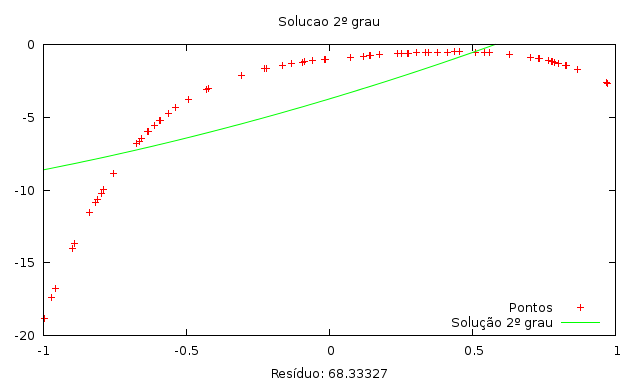
\includegraphics[scale=0.7]{sol2grau}
\end{figure}

Ao perturbar os dados de entrada em 15\%, o programa calculou as funções 
com resíduos 80.79981 para perturbação em $b$ e 88.55303 para perturbação em $A$ e $b$.

\begin{figure}[h]
\centering
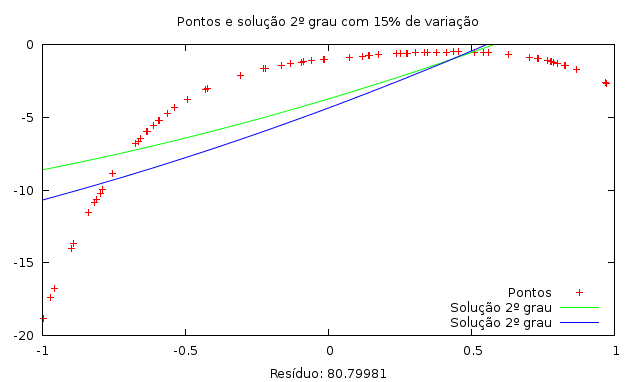
\includegraphics[scale=0.7]{sol2grau_var}
\end{figure}


\newpage
\section{Solução 3º grau}

Ao buscar uma função mônica de grau 3 para aproximar os pontos encontrou-se os seguintes 
coeficientes:

\(x_0 = -0.39367  ,~  x_1 = 5.45203  ~$e$~ x_2 = -9.03908 \)

\begin{figure}[h]
\centering
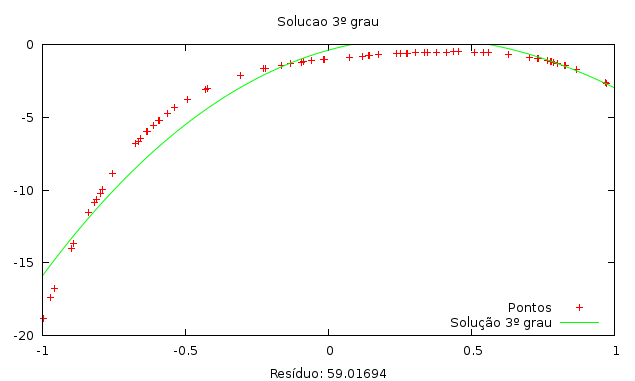
\includegraphics[scale=0.7]{sol3grau}
\end{figure}

Ao perturbar os dados de entrada em 15\%, o programa calculou as funções 
com resíduos 69.37743  para perturbação em $b$ e 68.57657 para perturbação em $A$ e $b$.
\begin{figure}[h]
\centering
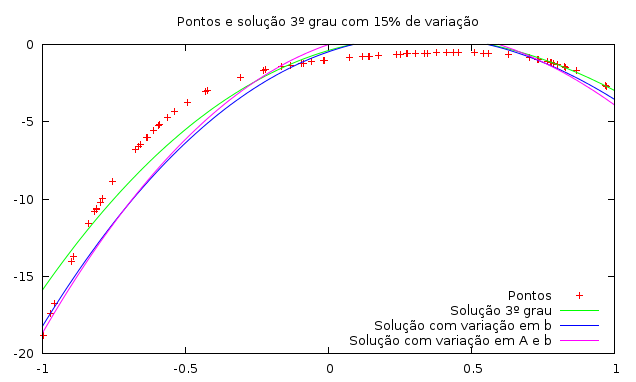
\includegraphics[scale=0.7]{sol3grau_var}
\end{figure}

\newpage
\section{Solução 4º grau}

Ao buscar uma função mônica de grau 4 para aproximar os pontos encontrou-se os seguintes 
coeficientes:
\(x_0 = -0.34728 ,~  x_1 = 1.25949,~ x_2 =  -8.95480 ~$e$~ x_3 = 6.95427 \)

\begin{figure}[h]
\centering
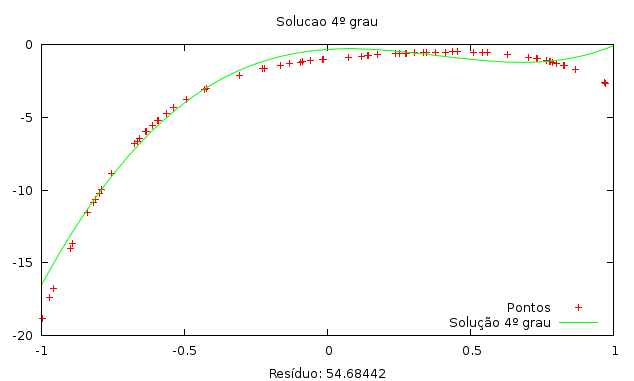
\includegraphics[scale=0.7]{sol4grau}
\end{figure}
Ao perturbar os dados de entrada em 15\%, o programa calculou as funções 
com resíduos 64.67217 para perturbação em $b$ e 56.54760  para perturbação em $A$ e $b$.
\begin{figure}[h]
\centering
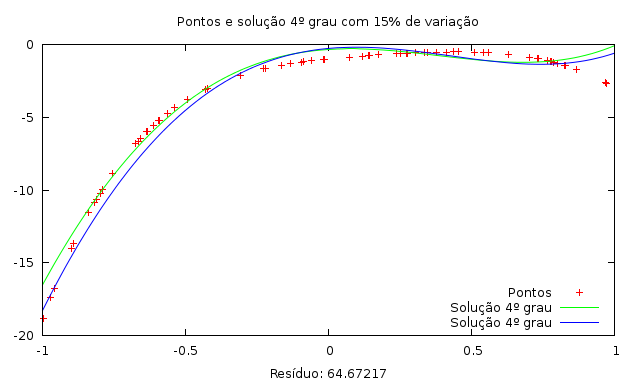
\includegraphics[scale=0.7]{sol4grau_var}
\end{figure}

\newpage
\section{Solução 5º grau}

Ao buscar uma função mônica de grau 5 para aproximar os pontos encontrou-se os seguintes 
coeficientes:

\(x_0 = -0.99223,~    x_1 = 1.73653,~x_2 = -2.98373,~ x_3 = 6.13233 ~$e$~ x_4 =  -7.05190 \)

\begin{figure}[h]
\centering
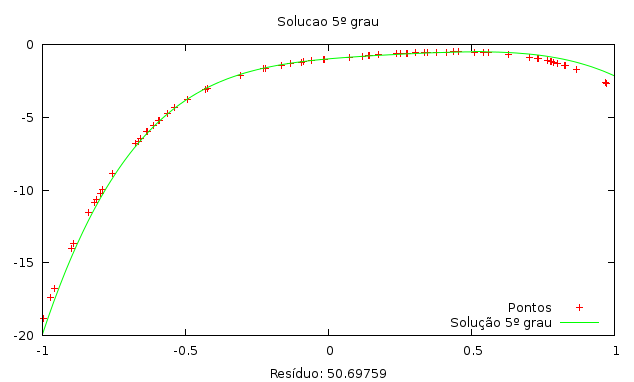
\includegraphics[scale=0.7]{sol5grau}
\end{figure}
Ao perturbar os dados de entrada em 15\%, o programa calculou as funções 
com resíduos 61.44919  para perturbação em $b$ e 47.96817 para perturbação em $A$ e $b$.
\begin{figure}[h]
\centering
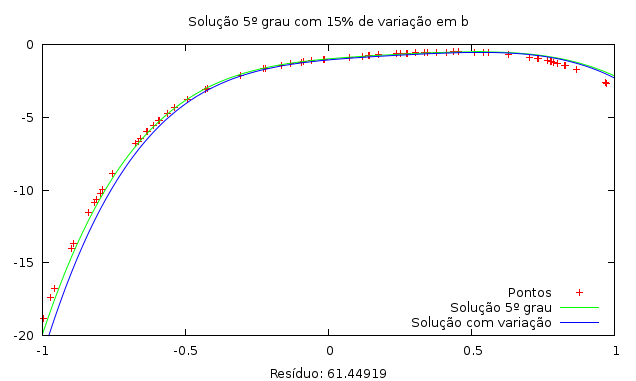
\includegraphics[scale=0.7]{sol5grau_var}
\end{figure}

Note que a o resíduo ($||s||$) aumenta cada vez que o grau da solução do polinômio diminui. Isto indica que o 'erro’ da aproximação está sendo cada vez maior.\footnote{Observação: estes testes podem ser realizados com os arquivos matgrau5.txt, matgrau4.txt, matgrau3.txt, matgrau2.txt.}

